\chapter{Project Schedule}

%This section describes the project’s planned schedule or timeline and how the project measured against this plan.  This information is helpful in identifying and understanding what may have contributed to project delays or allowed the project to complete early or on time.  This can then be used by the team members on future projects or be referenced by other project teams for use on future projects.  Archiving project information during the project closure phase is one of the best ways for an organization to improve its project management methodologies and effectiveness. 

This bachelors project was scheduled for six months with initiation date on Januray 1st, 2017 and completion date 2nd June, 2017. The time-line of the project is represented by the milestones. Completion of all the milestones will be a measure of the projects success. \bigskip

Fig. \ref{fig:timeline} shows the time-line of the project with the milestones marked in green when reached. 

\begin{figure}[H]
          \centering
            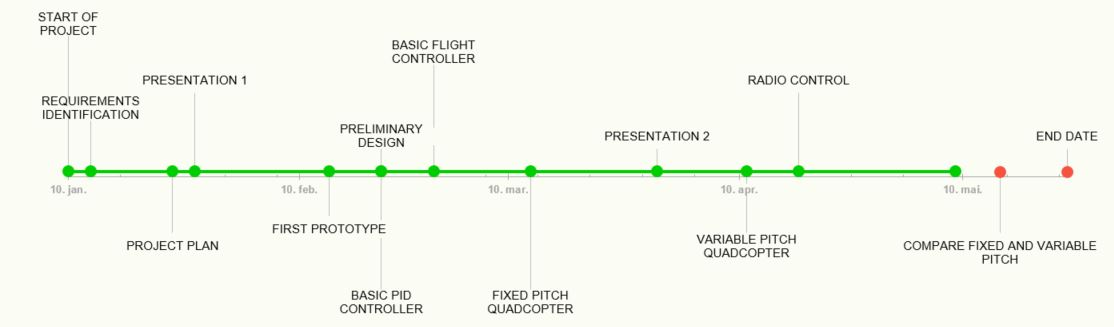
\includegraphics[scale = 0.6]{VAPIQ-PICTURES/Timeline}
                \caption{Timeline of The Project}
                \label{fig:timeline}
            \label{dir}
\end{figure}    


\section{Planning}

For planning the project, a combination of traditional planning using Gantt chart and Scrum planning was used. The Gantt chart is provided in Appendix \textbf{\ref{app:gantt}}. Making the Gantt chart in full detail in the initial phase of the project was challenging. In this phase the team had little experience with both project planning and quadcopters. \bigskip

Due to the nature of this project, rapid prototyping has been essential. If the team was to execute research and testing on a variable pitch quadcopter within the given time-frame, the quadcopter and flight controller had to be made in the shortest possible time. This gave the team little time to elaborate in the early phases of the project which led to a more trial and error approach with fast adaptations using Scrum. \bigskip

Scrum ceremonies like daily Scrum, sprint planning and retrospective meetings have helped the team identify what worked and what did not work. In this way, pitfalls have been identified and progress has been made.\bigskip

In retrospect, many things could have been done differently based upon the knowledge acquired throughout the project cycle. \bigskip

The process of creating two types of flight controllers, an autonomous system, two quadcopters and then testing it all, is a huge undertaking. The task of completing all these objectives in the given time-frame was underestimated and the team did to some extent overcommit.
%If we had known in advance were the pitfalls and time thives were 

\clearpage

\section{Deliverables} 

For this project the Norwegian Defence Research Establishment(FFI) wanted the students to investigate the characteristics and benefits of variable pitch for use on quadcopters. The objectives were:

\begin{itemize}
    \item Build a small quadcopter ($<2,5 kg$) with variable pitch 
    \item Build a small quadcopter ($<2,5 kg$) with fixed pitch
    \item Investigate if variable pitch gives the possibility of more stable flight and landing in turbulent conditions
    \item Investigate if variable pitch improves response time
    \item Compare the fixed pitch quadcopter against the variable pitch quadcopter
\end{itemize}

Many of the objectives have been completed, but some are still in partial fulfillment. Many activities have taken more time than planned and multiple unforeseen events have taken place. \\

Due to delays and unforeseen events, less time has been used for fine tuning and testing of the variable pitch quadcopter than initially intended. If the team had chosen a different approach, it is plausible that the team could have gotten to the point of research at an earlier stage. On the contrary, the way that was chosen has given a tremendous learning outcome for all participants.\\

The objectives in partial fulfillment are; 
\begin{itemize}
    \item The fixed pitch quadcopter was made, but did not work as intended and was discarded. Instead the variable pitch quadcopter was used in fixed pitch mode for comparison.
    \item The investigation of stability on variable pitch quadcopters have not been fully fulfilled. This is due to the work that was required to achieve a sufficiently stable quadcopter.
    \item Landing tests have been performed, but not autonomously. The autonomous control with Qualisys has been developed but has never been fully tested due to lack of time.
    \item The comparison part of the objectives is executed but not to the full extent initially intended. This has also been due to lack of time. 
\end{itemize}


\section{Budget}
The project was given a total budget of 15.000 NOK. The budget was intended to cover all expenses related to the project. The budget was overran in sprint 8 when the need for new variable pitch mechanisms occurred.\bigskip

The main part of the expenditures relates to procurement of motors and variable pitch mechanisms, and electronics. Most of the components and parts were ordered from abroad, so additional expenses came with shipping and customs. All the expenses are documented and all receipts are kept for the customer. \bigskip

The total amount spent in the project sums up to: 15.437 NOK.